\chapter{Méthodes expérimentales}

\section{pix2pix avec PASCAL}

Nous avons implémenté le modèle pix2pix sur un sous ensemble de données d'image prévenant de la dataset Pascal, cet ensemble contient 2913 paires d'images (image d'origine et segmenté) sur 20 classes différentes :
\begin{itemize}
	\item Personne : personne 
	\item Animal : oiseau, chat, vache, chien, cheval, mouton
	\item Véhicule : avion, bicyclette, bateau, bus, voiture, moto, train
	\item Intérieur : bouteille, chaise, table à manger, plante en pot, canapé, télévision/moniteur
\end{itemize}

Comme la plupart des utilisateurs de pix2pix sont basées sur des jeux de données à une classe, tels que le visage, la façade…etc. Nous menons des expériences sur le jeu de données qui a une scène plus complexe, qui souvent contient plus d'une classe dans une image, par exemple :


\begin{figure}[H] 
	\centering 
	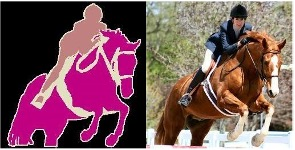
\includegraphics[width=0.5\textwidth]{./resources/img/im_pascal.jpg} %插入图片,[]中设置图片大小,{}中是图片文件名
	\caption{Image segmenté et image d'origine contenant une personne et un cheval} %最终文档中希望显示的图片标题
	\label{Fig4_1} %用于文内引用的标签
\end{figure}


\newpage
 Nous avons effectué notre expérience sur le pix2pix en trois parties :
 
 \begin{enumerate}[label=(\alph*)]
 	\item Sur les voitures
 	
 	Tout d'abord, nous avons mené notre expérience sur le sous-ensemble de données qui contient principalement que des voitures. Après 200 époques d'apprentissage avec une taille de lot de 1, le modèle est capable de générer le profil général d'une voiture, et il est capable de remarquer la position des pneus et des fenêtres. De plus, comme la plupart des voitures dans l'ensemble du jeu de données sont noirs et rouge, et pix2pix est un GAN basé sur la théorie statique. Les voitures générées sont principalement en noir avec un mélange de rouge. (Exemple en annexe).
 	
 	
 	\item Sur toute les images avec leurs arrière-plans
 	
 	Deuxièmement nous avons nous avons mené l'expérience avec toute des images, et la plupart de ces images présente des scènes complexes avec plusieurs classe en même temps. Après 400 époques d'apprentissage avec une taille de lot de 1, Malgré que la classe personne est la plus redondante dans nos images, il est difficile de générer une personne réelle à partir de l'image d'entrée. Et pour certaines classes simples comme les avions, vélos, bus et les bateaux qui apparaissent souvent dans des scènes monotones (ciel, routes, mer…etc.), le modèle est capable de générer un objet très similaires à un objet réel. (Exemple en annexe).
 	
 	\item Sur toute les images sans leurs arrière-plans
 	
 	
 	Enfin, nous avons expérimenté sur l'ensemble des images en augmentant le nombre des images par la duplication (miroir et rotation) et en enlevant l'arrière-plan afin de savoir si l'arrière-plan influence. L'une des raisons est que les scènes ou les personnes apparaissent sont très variées et après 300 époques d'entrainement avec une taille de lot de 1, nous avons générer des images (Exemple en annexe). Et nous avons observé qu'il n'y a pas de d'amélioration par rapport à l'étape avec les images contenants l'arrière-plan.
 	
 \end{enumerate}

À la fin de ces expériences nous avons dessiné les graphes de loss afin d'observer le comportement de la loss du générateur et notamment la loss du discriminateur. Nous notons que le D{\_}real avec la ligne verte signifie la loss du discriminateur pour les images réelles, le D{\_}fake signifie la loss du discriminateur pour les images fausses g.n.r.es enfin nous avons G{\_}GAN qui signifie la loss du générateur pour les images fausses. Nous notons aussi que la stabilité de notre modèle est liée à la stabilité des loss de D{\_}real, D{\_}fake et G{\_}GAN.

\begin{figure}[H] 
	\centering 
	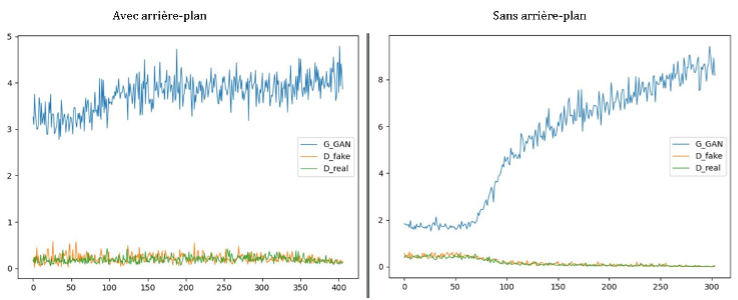
\includegraphics[width=1.0\textwidth]{./resources/img/im_pascal_loss.png} %插入图片,[]中设置图片大小,{}中是图片文件名
	\caption{Graphe de loss de pix2pix avec les images contenant un arrière-plan et non.} %最终文档中希望显示的图片标题
	\label{Fig4_2} %用于文内引用的标签
\end{figure}

Nous remarquant que notre modèle avec des images contenant un arrière-plan est stable car G{\_}GAN, D{\_}fake et D{\_}real sont stable. Et pour le modèle avec les images sans arrière-plan, il est stable jusqu'à l'époque 75, puis devient instable car la loss de G{\_}GAN augment énormément.
Nous avons aussi appliqué le modèle avec l'arrière-plan sur des images qui ne contiennent pas d'arrière-plan afin le modèle permet de générer un arrière-plan presque parfait pour certaines classes par exemple pour les avions il génère le ciel, pour les animaux il génère la verdure (Exemple en annexe).


\section{Espace latent de BigGAN}

Après avoir fini l'étape 1 ou nous avons obtenu des résultats pas très satisfaisants sur la génération des images similaires, nous nous sommes redirigés vers l'étude de BigGAN.  Dans cette partie nous avons expérimenté BigGan de DeepMind, ce GAN a été entrainé sur l'imageNet qui contient 1000 classes différentes. Il a été entrainé à une résolution de 128*128, 256*256 et 512*512. Nous avons utilisé le modèle avec la résolution de 128*128.

Nous avons fait deux expériences pour cette partie qui sont :

1.	Nous fixons la classe et nous changeons le bruit.

2.	Nous changeons la classe et le bruit.

\subsection{Expérience 1}
Pour la première expérience dans cette étape nous commençons par générer l'image target au hasard ensuite nous allons fixer le vecteur de classe encoder en one-hot et nous changeons le bruit en l'optimisant avec les loss en utilisant la descente de gradient stochastique Adam.

\begin{algorithm}[H]
	
	\SetAlgoLined
	\KwInput{une image target $I_0$}\;
	\KwResult{imge $I_final$ le plus ressemblant à $I_0$ }
	$ n = 1 $
	
	Donner un vecteur de bruit aléatoirement
	
	\For{$n < $ numbre d'iteration}{Générer Image $I_n$ par BigGAN avec le vecteur de bruit  \\ Calcule de la loss sémantique L2 entre $I_0$ et $I_n$ (replace classify block de squeezenet by a flatten layer) \\ Calcule de la loss pixel entre $I_0$ et $I_n$ \\  loss $=$ $-$ loss sémantique + 30*loss pixel (on se focalise beaucoup plus sur la loss pixel pour cette étape)  \\  faire backpropagation et optimiser le vecteur de bruit 
		
	}
\caption{vecteur de classe fixe}
\end{algorithm}

Nous avons appliqué notre algorithme sur 4 exemples (les images cadré en rouge sont des images but et les images cadré en vers sont le résultat final et les autres sont les étapes intermédiaires.)

L'exemple 1 nous avons essayé de générer un tigre à partir d'un chat sans changer la classe, en optimisant que le bruit.
\begin{figure}[H] 
	\centering 
	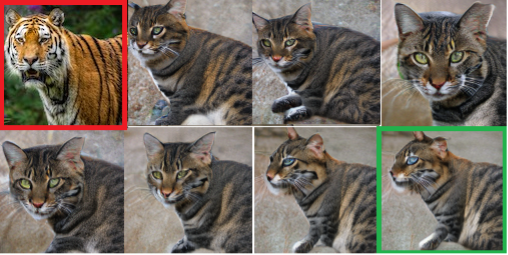
\includegraphics[width=0.8\textwidth]{./resources/img/cat2tiger_0.png} %插入图片,[]中设置图片大小,{}中是图片文件名
	\caption{Chat vers le tigre} %最终文档中希望显示的图片标题
	%\label{Fig4_2} %用于文内引用的标签
\end{figure}

L'exemple 2 nous avons essayé de générer un TGV à partir d'un camion sans changer la classe, en optimisant que le bruit.
\begin{figure}[H] 
	\centering 
	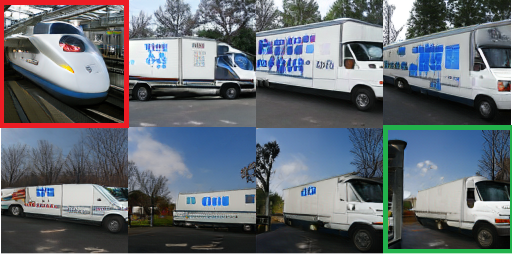
\includegraphics[width=0.8\textwidth]{./resources/img/car2train_0.png} %插入图片,[]中设置图片大小,{}中是图片文件名
	\caption{Camion vers train } %最终文档中希望显示的图片标题
	%\label{Fig4_2} %用于文内引用的标签
\end{figure}

L'exemple 3 nous avons essayé de générer un chien à partir d'un chat sans changer la classe, en optimisant que le bruit.
\begin{figure}[H] 
	\centering 
	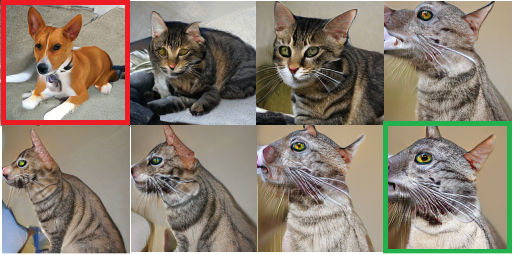
\includegraphics[width=0.8\textwidth]{./resources/img/cat2dog_0.png} %插入图片,[]中设置图片大小,{}中是图片文件名
	\caption{chat vers chien} %最终文档中希望显示的图片标题
	%\label{Fig4_2} %用于文内引用的标签
\end{figure}

L'exemple 4 nous avons essayé de générer une voiture à partir d'un chien sans changer la classe, en optimisant que le bruit.
\begin{figure}[H] 
	\centering 
	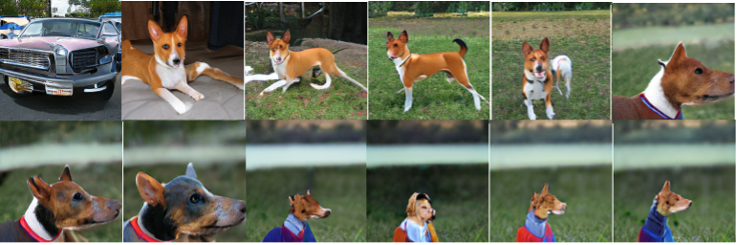
\includegraphics[width=1.0\textwidth]{./resources/img/dog2car_0.png} %插入图片,[]中设置图片大小,{}中是图片文件名
	\caption{chien vers voiture} %最终文档中希望显示的图片标题
	%\label{Fig4_2} %用于文内引用的标签
\end{figure}

\subsection{Expérience 2}
Pour la deuxième expérience dans cette étape nous commençons par générer l'image target au hasard ensuite nous allons changer le vecteur de classe et le bruit en les optimisant avec la descente de gradient stochastique Adam, et vu que le vecteur de classe est encoder en one-hot nous allons le transformer avec la fonction softmax afin qu'il puisse être optimisé.

\begin{algorithm}[H]
	
	\SetAlgoLined
	\KwInput{une image target $I_0$}\;
	\KwResult{imge $I_final$ le plus ressemblant à $I_0$ }
	$ n = 1 $
	
	Donner un vecteur de bruit aléatoirement
	
	Donner un vecteur de classe en forme de one hot coding
	
	\For{$n < $ numbre d'iteration}{vecteur de classe = softmax(vecteur de classe) \\ Générer Image $I_n$ par BigGAN avec le vecteur de bruit et le vecteur de classee   \\ Calcule de la loss sémantique cosine entre $I_0$ et $I_n$ (replace classify block de squeezenet by a flatten layer) \\ Calcule de la loss pixel entre $I_0$ et $I_n$ \\  loss $=$ $-100*$ loss sémantique + 30*loss pixel \\  faire backpropagation et optimiser le vecteur de bruit et le vecteur de classe
		
	}
	\caption{vecteur de classe non fixe}
\end{algorithm}

Nous avons appliqué notre algorithme sur 3 exemples (les images cadré en rouge sont des images but et les images cadré en vers sont le résultat final et les autres sont les étapes intermédiaires).

L'exemple 1 nous avons essayé de générer un tigre à partir d'un chat en optimisant la classe et le bruit.
\begin{figure}[H] 
	\centering 
	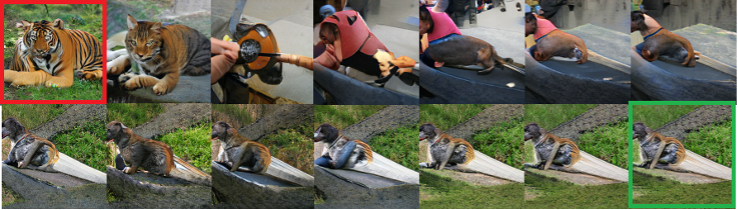
\includegraphics[width=0.9\textwidth]{./resources/img/cat2tiger_1.png} %插入图片,[]中设置图片大小,{}中是图片文件名
	\caption{Chat vers tigre} %最终文档中希望显示的图片标题
	%\label{Fig4_2} %用于文内引用的标签
\end{figure}

L'exemple 2 nous avons essayé de générer un chien à partir d'un chat en optimisant la classe et le bruit.
\begin{figure}[H] 
	\centering 
	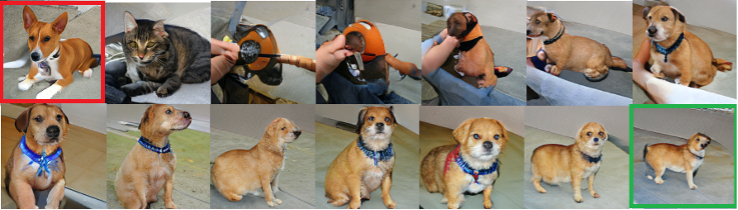
\includegraphics[width=0.9\textwidth]{./resources/img/cat2dog_1.png} %插入图片,[]中设置图片大小,{}中是图片文件名
	\caption{Chat vers chien} %最终文档中希望显示的图片标题
	%\label{Fig4_2} %用于文内引用的标签
\end{figure}

L'exemple 3 nous avons essayé de générer une voiture à partir d'un chien en optimisant la classe et le bruit.
\begin{figure}[H] 
	\centering 
	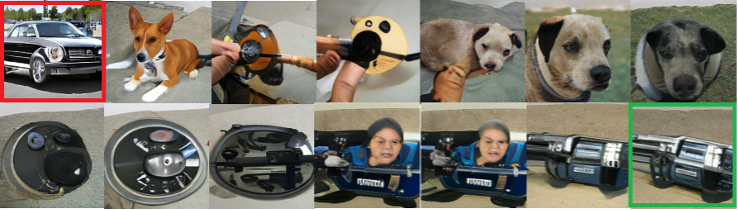
\includegraphics[width=0.9\textwidth]{./resources/img/dog2car_1.png} %插入图片,[]中设置图片大小,{}中是图片文件名
	\caption{Chien vers voiture} %最终文档中希望显示的图片标题
	%\label{Fig4_2} %用于文内引用的标签
\end{figure}

Nous remarquant que quand on fixe la classe et on optimise juste le bruit notre modèle converge vers quelque chose de similaire à notre image but, sauf si les deux classes qui se ressemble (chien vers chat, chat vers tigre, camion vers train..etc)

Nous remarquant que quand nous optimisant le bruit et le vecteur de classe nous avons beaucoup d'objets déformer sans aucun sens qui se génèrent et on converge généralement vers une image qui est complétement différente à notre image but. 

Un principale raison est que dans l'architecture de BigGAN, le classe vecteur n'existe que dans l'espace latent, il est connecté à plusieurs intermédiaire layer, voire il est une variable de haute dimension. Cela apport la labilité sur l'optimisation. Et l'autre raison vient de softmax fonction, étant donnée qu'il y a un mile classes, après avoir utilisé softmax sur one hot coding, la classes vecteur devient (0.001,  0.001, ...), qui mal initialise le vecteur au début de l'optimisation. Et face à cette problème, on a aussi essayé retourner la classes vecteur à la forme one hot coding lord d'entrer à BigGAN, en assurant l'usage de autograd de Pytorch. On a utilisé le gumbel softmax qui peut-etre approprié. Cependant, il demande trop d'itération pour être convergé et il rend le processus de l'optimiser le vecteur de classe extrêmement aléatoire puisque c'est une variable de mile dimension.

\subsection{Expérience supplémentaire, Singe ver Einstein}

\begin{figure}[H] 
	\centering 
	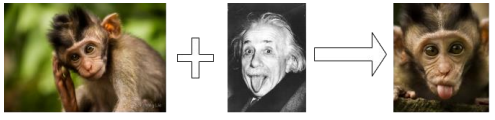
\includegraphics[width=0.9\textwidth]{./resources/img/enoce.png} %插入图片,[]中设置图片大小,{}中是图片文件名
	\caption{exemple but } %最终文档中希望显示的图片标题
	%\label{Fig4_2} %用于文内引用的标签
\end{figure}

En fait toutes les expérience ont faites dans le cadre de ImageNet, c'est à dire que toutes images target et images généré sont de ImageNet. Donc, on pense à faire une expérience supplémentaire, qui est dehors ImageNet.  Nous avons donc essayé d'obtenir le résultat de la figure 10 qui est présente sur l'énoncé du sujet, et cela en utilisant l'algorithme 2 et nous avons obtenu le résultat de la figure 11. 

\begin{figure}[H] 
	\centering 
	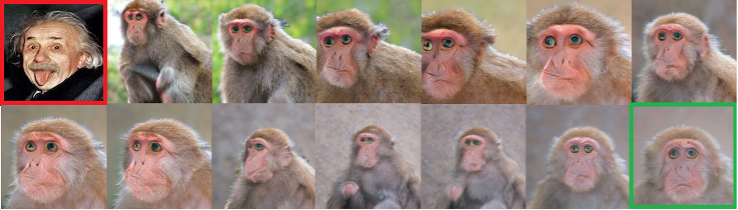
\includegraphics[width=0.9\textwidth]{./resources/img/singe2einstein.png} %插入图片,[]中设置图片大小,{}中是图片文件名
	\caption{Singe vers Einstein} %最终文档中希望显示的图片标题
	%\label{Fig4_2} %用于文内引用的标签
\end{figure}

Nous remarquons que sur les images des étapes intermédiaires il essaie de générer une tête similaire à celle d'Einstein  en générant les mêmes cheveux au niveau de son oreille et aussi il essaie de trouver comment créer la langue. Malheureusement il ne pourra pas faire cela et vers la fin nous remarquons que l'émotion d'Einstein et le singe sont différentes.










